\documentclass[a4paper,12pt,twoside]{book}
\usepackage{lesi/lesi}

\title{Título do Relatório}
\author{Nome do Autor}
\nrAluno{12345}
\regimeDiurno         % ou \regimePosLaboral
\LESI
\date{2019/2020}

%% Caso tenham mais que um orientador, colocar
%% \orientador{Nome professor \AND Nome professor}
\orientador{Nome do Professor}

%% comentar estas três linhas para projectos
\empresa{The Great Team}
\enderecoEmpresa{Braga, Portugal}
\supervisor{Eng. A. U. Thor}

% comentar se não for para usar glossários
\makeglossaries




\begin{document}
\frontmatter
\maketitle  % print the title


\begin{resumo}
Resumo do trabalho realizado. Deve ser sucinto, e cobrir todo o relatório: uma introdução ao problema que se pretendeu resolver, um pequeno resumo da abordagem realizada, e algumas conclusões do trabalho atingido.

Poderão ser criados vários parágrafos, até para que cada um corresponda às três fases de introdução, desenvolvimento e conclusão.

Não é relevante colocar no resumo o local de estágio ou a referência ao curso. 
\end{resumo}

\begin{abstract}
This is the translation of the previous text. It should say the exact same thing. Please do not use directly Google Translator.
\end{abstract}

%% Comment the following part if you are not acknowledging anybody
\begin{agradecimentos}
[A secção de agradecimentos é a parte pessoal do documento, e o único sítio onde o aluno pode escrever de forma menos formal, usando o tipo de linguagem que lhe parecer adequado para as pessoas a quem agradece.]
\end{agradecimentos}


\tableofcontents

% comentar se nao tiver figuraIs
\listoffigures

% comentar se nao tiver tabelas
\listoftables

% comentar se nao se quiser lista de listagens
\lstlistoflistings

% Commentar proximas duas linhas se nao for para usar acronimos

\newacronym{php}{PHP}{HyperText Preprocessor }

\newacronym{sql}{SQL}{Structured Query Language}

\newacronym{xampp}{XAMPP}{Cross-Plataform(X), Apache(A), MariaDB(M), PHP (P) e Perl (P)}

\newacronym{moscow}{MoSCoW}{Must Have, Should Have, Could Have, Won't Have}

\newacronym{html}{HTML}{HyperText Markup Language}

\newacronym{wysiwyg}{WYSIWYG}{\textit{What You See Is What You Get}}

\printglossary[type=\acronymtype,title={Siglas \& Acrónimos}]

% Commentar proximas duas linhas se nao for para usar glossarios



\newglossaryentry{moscow}
{
   name=MoSCoW,
   description={Método de priorização de funcionalidades ou requisitos }
}


\newglossaryentry{stemmer}
{
    name=stemmer,
    description={Ferramenta capaz de reduzir uma palavra à sua raiz. Por exemplo, para a palavra ``correria'', a sua raiz seria ``corre''. }
 }

\printglossary


\printglossary


\mainmatter


\chapter{Introdução}

%[A introdução deve, tal como o próprio nome indica, introduzir o tema do trabalho. Não deve haver pressa em falar da empresa onde foi realizado o estágio ou o curso a que se refere o trabalho. Deve fazer-se uma introdução à área, Os Sistemas Informáticos ou as Ciências da Computação são áreas bastante grandes, pelo que não se deve supor que o leitor está a par das necessidades ou das tecnologias usadas em determinada área. No entanto, não devem ser explicados conceitos básicos, que qualquer licenciado numa engenharia de sistemas informáticos ou em ciências da computação tenham obrigação de conhecer.

Acompanhar as novas tecnologias é fundamental para um negócio. É preciso investir em inovação para manter um negócio no mercado competitivo. A tecnologia, aliada a uma boa atualização, consegue proporcionar soluções eficientes às empresas.

% Algo como o resumo é valido para a introdução ???
-- por terminar -- acabaram as ideias !!

\section{ Objetivos }

% - [Numa pequena secção da introdução liste, cuidadosamente, os objetivos do trabalho. Não confundir com os requisitos do software. Apenas o que se pretendia atingir originalmente.] %

Este estágio está diretamente relacionado com o produto NkaAcademies, que se trata de uma solução web completa para a gestão de processos de formação.

%1ª opçao
%Deste modo, os principais objetivos estipulados foram a migração completa do produto NkaAcademies para as versões mais recentes do PHP e do MySQLi e posteriormente o desenvolvimento de novas funcionalidades.

%2ª opçao
Pretende-se efetuar a migração completa do produto NkaAcademies para as versões mais recentes do PHP e do MySQLi,no entanto será necessário resolver alguns problemas de compatibilidade que poderão surgir consequentemente a esta alteração e numa fase mais avançada do estágio, incorporar novas funcionalidades ao produto.

\section{Contexto}
 %[No caso de um estágio, é nesta secção que se deverá falar da empresa em que o estágio foi realizado. Se o projeto desenvolvido faz parte de um projeto mais amplo, faz sentido que se documente os objetivos do projeto com um todo, de modo que o leitor consiga perceber onde o trabalho realizado encaixa.] %
\par Este projeto foi realizado no âmbito de estágio curricular da Licenciatura em Engenharia de Sistemas Informáticos, na empresa NKA - \textit{New Knowledge Advice} em Braga.
\par O estágio curricular teve uma duração de aproximadamente quatro meses, tendo iniciado a 22 de fevereiro e terminado a 9 junho de 2021, de segunda a quinta feira num regime maioritariamente de teletrabalho, com exceção de algumas semanas em regime presencial.
\par A NKA - \textit{New Knowledge Advice} é uma empresa tecnológica sediada em Braga, fundada em 2011 que concebe e desenvolve soluções globais vocacionadas para a otimização de cada negócio, por meio de projetos específicos, fornecendo as soluções mais adequadas às crescentes exigências dos mercados. A empresa dedica-se ainda ao desenvolvimento de software, à implementação de sistemas e à consultoria e formação. % incluir ref ao site da nka (??)

\section{Plano de trabalhos}

No âmbito do estágio, foram identificadas as seguintes tarefas:

\begin{itemize}
    \item  Conhecer a empresa, tecnologias e projeto a desenvolver - Migração do produto NkaAcademies para as versões mais recentes do PHP e MySQLi;
    \item  Investigação sobre PHP e MySQLi - Leitura de CHANGELOG das versões anteriores. Análise de funções \textit{deprecated}.
    \item  Alteração do código para a versão 8 PHP.
    \item  Testes e correção de erros de compatibilidade
    \item  Conhecer o projeto a desenvolver - módulo auxiliar ao processo de gestão de formação.
    \item Levantamento de requisitos e funcionalidades
    \item  Desenvolvimento do módulo - Filtro de pesquisa e alteração manual e automática de documentos associados à gestão de formação.
    \item Testes e correção de erros
    \item  Preparação da aplicação - Alteração de ligações para cloud. Limpeza de código.
    \item Atualização das alterações no servidor
\end{itemize}
Para planear a execução das tarefas, foi elaborado um diagrama de Gantt de acordo com a Figura - ~\ref{fig:gantt}.

\begin{center}
        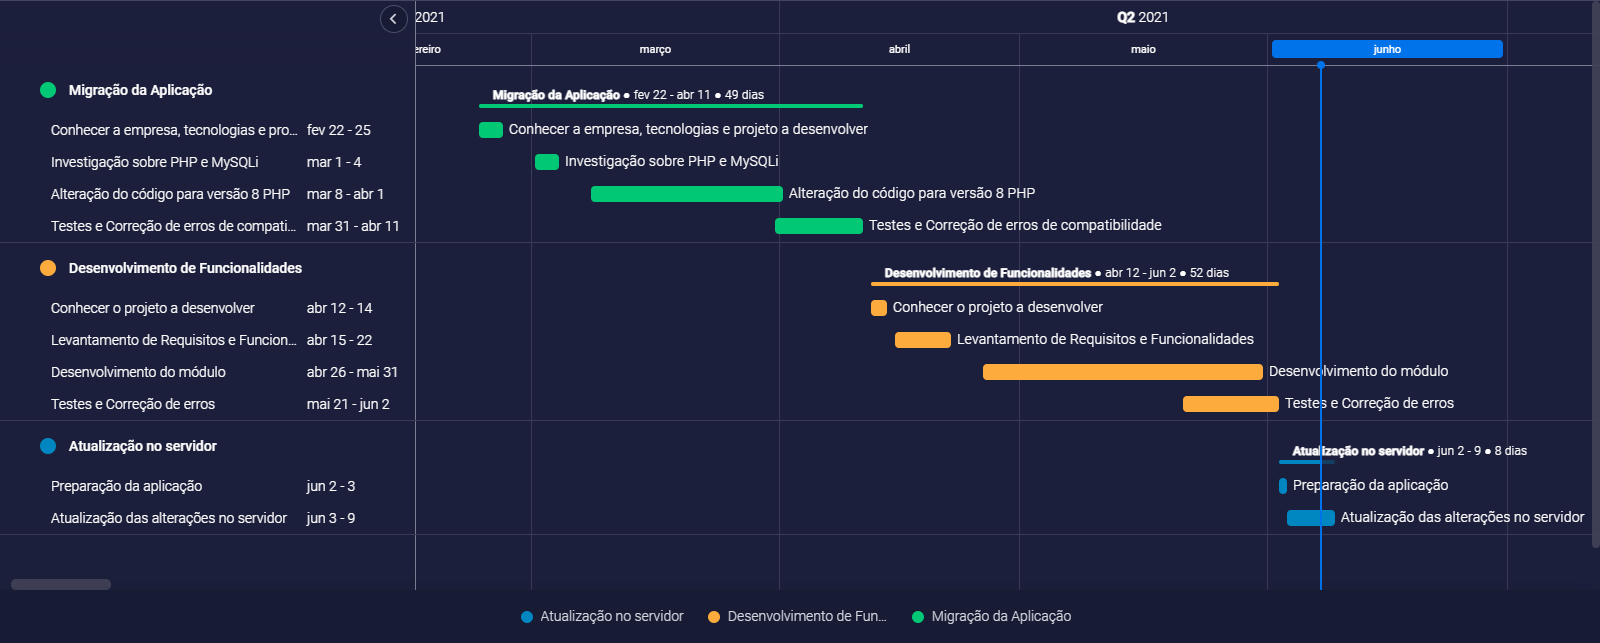
\includegraphics[width=\textwidth,height=\textheight,keepaspectratio]{images/gantt.png}
        \captionof{figure}{Diagrama de Gantt}
        \label{fig:gantt}
\end{center}


\section{Estrutura do documento}
 [A última secção da introdução deve explicar a estrutura do documento: quais são só capítulos existentes (para além do primeiro) e o que será discutido em cada um desses capítulos. A estrutura típica de um relatório de desenvolvimento de software é:

 Introdução, com um breve resumo do que se pretende atingir, e uma descrição clara dos objetivos;

\begin{enumerate}
    \item Análise ao problema, que poderá incluir uma análise ao estado da arte ou ao modelo de negócio onde se pretende intervir;
    \item Análise e modelação do sistema, em que sejam levantados sistematicamente os requisitos, descritos diagramas de caso de uso e de atividade (que descrevam/formalizem o modelo de negócio).
    \item Implementação, em que se descrevam as tecnologias escolhidas (e se justifiquem), e se refira detalhes sobre a implementação.
    \item Análise de resultados e testes, seja uma análise/avaliação aos resultados obtidos, sejam testes de usabilidade ou unitários ao trabalho desenvolvido.
    \item Conclusão.]
\end{enumerate}{}


\chapter{Processo de Reengenharia}
\label{migracao}

A área da reengenharia de software está ligada à restruturação e redocumentação do software para o tornar mais fácil de perceber e alterar.

A funcionalidade do software não é alterada, e normalmente, não devem ser feitas grandes alterações a nível da arquitetura do sistema \citep{somerville}.

Neste capítulo estão descritas as principais tecnologias e plataformas utilizadas no desenvolvimento quer da primeira e segunda parte do estágio. São ainda enunciadas algumas funcionalidades e capacidades do produto NkaAcademies que vai ser alvo de alteração tecnológica. Por fim, são descritas sucintamente as melhorias a realizar no produto e são demonstrados alguns exemplos das alterações realizadas, tais como um "frente a frente"  de algumas funções suportadas nas diferentes versões do \acrshort{php} e um \textit{improvement} de funções.

%-- Texto
% tecnologias utilizadas, melhorias a realizar, funcionalidades e capacidades do produto, alteraçoes feitas com exemplos

\section{Descrição das Tecnologias e Plataformas}
\label{tecnologias}
Neste ponto serão descritas as tecnologias e plataformas utilizadas ao longo deste trabalho, tais como \acrshort{xampp}, Laragon, Visual Studio Code.

Para a realização deste projeto foram utilizadas as plataformas e tecnologias requeridas pela empresa para facilitar a implementação e integração do projeto, e para tal foi necessário proceder à sua aprendizagem.

De seguida vão ser descritas de forma sucinta as tecnologias e plataformas utilizadas ao longo do projeto.\newline


\textbf{XAMPP}

O \acrshort{xampp} é formado por um pacote que inclui, base de dados MySQL, servidor web Apache e interpretadores para as linguagens de script. É essencialmente utilizado pelos desenvolvedores que pretendem criar um servidor web local no seu próprio computador, com a finalidade de realizar testes sem necessitar de acesso à rede \citep{xampp}.\newline


\textbf{Visual Studio Code}

O VsCode é um editor de código-fonte simplificado com suporte para operações de desenvolvimento como \textit{debugging}, execução de tarefas e controlo de versões \citep{vscode}.\newline % vs code FAQ - https://code.visualstudio.com/docs/supporting/FAQ

\quad \textbf{Xdebug}

\quad O Xdebug é uma extensão para \acrshort{php} que fornece uma variedade de recursos para melhorar a experiência de desenvolvimento de \acrshort{php} \citep{xdebug}.\newline


\textbf{Laragon}

O Laragon é uma maneira rápida e fácil de criar um ambiente de desenvolvimento isolado no Windows. Inclui Mysql, PHP Memcached, Redis, Apache \citep{laragon}.\newline

%----
\section{Listagem de Funcionalidades do produto}

NkaAcademies é uma solução web completa para a gestão de formação.
A solução é composta por vários módulos e diferentes funcionalidades, que fazem parte também de diferentes perfis. Existe então implementado no produto do NkaAcademies uma plataforma completa para a gestão de formações, para os professores/formadores e para os alunos/formandos, cada uma com diferentes propósitos que culminam num produto bem estruturado e completo \citep{nka1}.
%falar perfis, formador gestao formaçao e formando

Na \textbf{gestão da formação} (Figura ~\ref{fig:funcproduto}), algumas funcionalidades incluem:
\begin{itemize}
  \setlength\itemsep{-0.5em}
  \item Certificação de Diplomas
  \item Manuais Digitais
  \item Gestão de tarefas e projetos
  \item Faturação e gestão de recursos
  \item Cursos e-Learning
  \item Módulo de marketing
  \item Módulo de projetos
\end{itemize}

\begin{center}
        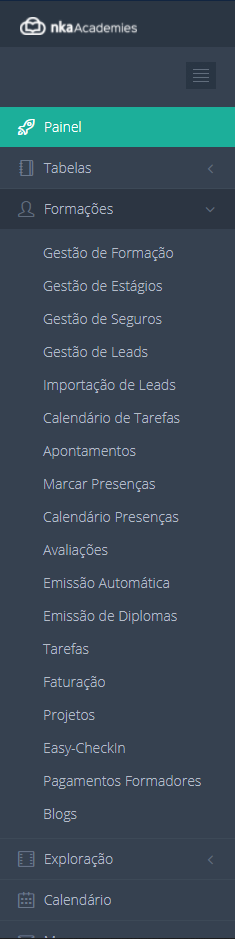
\includegraphics[width=\textwidth,height=0.5\textheight,keepaspectratio]{images/funcionalidades.png}
        \captionof{figure}{Gestão da Formação}
        \label{fig:funcproduto}
\end{center}

O produto é ainda composto por uma plataforma para os seus \textbf{formadores} onde poderão encontrar entre outras, as seguintes funcionalidades (Figura~\ref{fig:professor}):
\begin{itemize}
  \setlength\itemsep{0em}
  \item Presenças e avaliações online
  \item Listagem detalhada da turma
  \item Sistema interno de mensagens
  \item Partilhar apontamentos e exercícios
  \item Informação na "cloud" sincronizada
  \item Histórico de formações
\end{itemize}

\begin{center}
        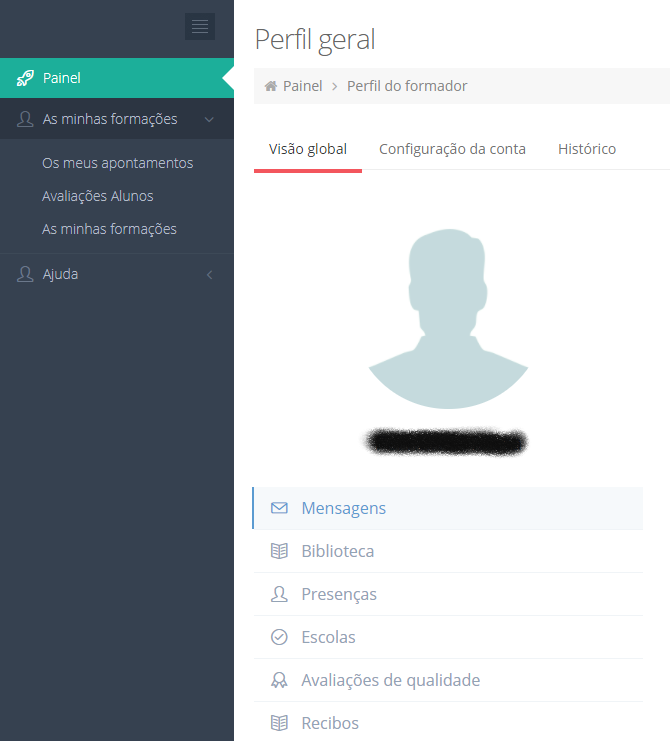
\includegraphics[width=\textwidth,height=\textheight,keepaspectratio]{images/professor.png}
        \captionof{figure}{Painel Formador/Professor}
        \label{fig:professor}
\end{center}

A plataforma disponibiliza também para os seus \textbf{alunos} e formandos um local onde poderão encontrar entre outras, as seguintes funcionalidades:
\begin{itemize}
  \item Partilha de diploma
  \item Descarregar manuais e documentos
  \item Devolver feedback
  \item Histórico de formação
  \item Manter o contacto com antigos colegas de formação
  \item Detalhes da formação
\end{itemize}

%---------------------
\section{Identificação das melhorias a realizar}

Atualmente, no mundo em que vivemos, \textit{updates} tecnológicos são lançados praticamente todos os dias relativos a sistemas de informação. É do maior interesse da parte de uma empresa, manter o seu produto atual e competitivo.

De momento, o produto NkaAcademies encontra-se desatualizado, utilizando versões antigas de \acrshort{php}(5.6) e MySQL. Foi então proposto desenvolver a migração de todo o produto NkaAcademies para as versões mais recentes, suportadas no \textit{host} utilizado pela empresa, do \acrshort{php}(5.6 -> 8.0.2) e do MySQL com o objetivo de atualizar o produto e também, em casos futuros o uso de novas funcionalidades que surgiram apenas em versões superiores à que o produto estava desenvolvido.

As melhorias a realizar passaram maioritariamente pela substituição total da biblioteca \acrshort{php} MySQL para MySQLi, uma vez que grande parte das funções que fazem parte da biblioteca MySQL foram descontinuadas / \textit{deprecated}, enquanto noutros casos apenas foram feitas alterações ao nível da chamada da função ou dos parâmetros (e ordem) recebidos. Posto isto, procedeu-se à sua alteração total no produto NkaAcademies, sendo que no caso de funções \textit{deprecated} foram implementadas alternativas \textit{hard-code} em \acrshort{php}.

Uma vez que se trata de uma migração completa de um produto pré-existente o objetivo principal definido para o cumprimento desta fase tem a ver com a compatibilidade das alterações feitas. As novas funções e todas as modificações realizadas ao nível do produto devem ser implementadas tendo em vista a sua compatibilidade com as versões anteriores, que neste caso são as versões \acrshort{php} 5.6 e 7 e a compatibilidade com outras funcionalidades já existentes no produto garantindo a operabilidade e o bom funcionamento da aplicação na nova versão tecnológica.
%%--

\section{Alterações no desenvolvimento da solução}

Neste capítulo serão apresentadas algumas das principais alterações implementadas no produto NkaAcademies na fase da migração da aplicação para as versões mais recentes do \acrshort{php} e MySQL.

As principais alterações efetuadas no projecto NkaAcademies foram ao nível da chamadas de funções, implementação de novos métodos devido à descontinuidade de funções da biblioteca MySQL, parâmetros (e ordem) recebidos por funções e correções de erros de compatibilidade entre versões.

\subsection{Comparação de funções}

Neste sub-capítulo serão comparadas as funções das bibliotecas MySQL e MySQLi, em relação a \textit{inputs} e \textit{outputs} de algumas das funções utilizadas.

\subsubsection{\textit{mysql\_select\_db vs mysqli\_select\_db}}

Neste caso, será apresentado um excerto de código relativo a uma função que foi atualizada na biblioteca MySQLi, recebendo o mesmo tipo de parâmetros mas que trocou a ordem de como eram incorporados na função.

A função \textit{mysql\_select\_db} (listagem~\ref{lst:6}) seleciona uma base de dados do tipo MySQL.

\begin{lstlisting}[language={php},
                   caption={Função mysql\_select\_db.},
                   label=lst:6]
function mysql_select_db($database, $link_identifier=NULL):bool

\end{lstlisting}

A função da Listagem~\ref{lst:6} recebe como argumentos:
\begin{itemize}
  \item \textbf{\$database}: nome da base de dados que deverá ser selecionada.
  \item \textbf{\$link\_identifier}: conexão ao MySQL.
\end{itemize}


A função \textit{mysqli\_select\_db} (listagem~\ref{lst:7}) seleciona a base de dados a ser utilizada ao realizar \textit{queries} do tipo MySQLi.

\begin{lstlisting}[language={php},
                   caption={Função mysqli\_select\_db.},
                   label=lst:7]
    	function mysqli_select_db($mysql, $database):bool

\end{lstlisting}

A função da Listagem~\ref{lst:7} recebe como parâmetros:
\begin{itemize}
  \item \textbf{\$mysql}: \textit{connection string} de acesso à base de dados.
  \item \textbf{\$database}: nome da base de dados que deverá ser selecionada.
\end{itemize}

%-----

\subsubsection{\textit{mysql\_result vs nka\_mysqli\_result}}

Neste exemplo será apresentado nos excertos de código a alteração que teve de ser feita quando a função da biblioteca MySQL não foi continuada na biblioteca MySQLi, fazendo com que tivesse de ser criada uma equivalente.

A função \textit{mysql\_result} (listagem~\ref{lst:4}) obtém os dados de um determinado resultado.

\begin{lstlisting}[language={php},
                   caption={Função mysql\_result.},
                   label=lst:4]
    	function mysql_result($result, $row, $field=0):string

\end{lstlisting}

A função da Listagem~\ref{lst:4} recebe como argumentos:
\begin{itemize}
  \item \textbf{\$result}: resultado da \textit{query} \acrshort{sql} a ser executado.
  \item \textbf{\$row}: número da linha do resultado.
  \item \textbf{\$field}: nome do campo a ser procurado (tabela).
\end{itemize}


A função \textit{nka\_mysqli\_result} (listagem~\ref{lst:1}), utilizada para substituir a função \textit{deprecated mysql\_result} foi implementada recebendo os mesmos argumentos que a anterior, e retornando uma \textit{string}.

\begin{lstlisting}[language={php},
                   caption={Função para substituir mysql\_result.},
                   label=lst:1]
      if (!function_exists('nka_mysqli_result')) {
      	function nka_mysqli_result($res, $row, $field=0) {
      	  $res->data_seek($row);
      	  $datarow = $res->fetch_array();
      	  return $datarow[$field];
      	}
      }
\end{lstlisting}

A função da Listagem~\ref{lst:1} recebe como argumentos:
\begin{itemize}
  \item \textbf{\$result}: resultado da \textit{query} \acrshort{sql} a ser executado.
  \item \textbf{\$row}: número da linha do resultado.
  \item \textbf{\$field}: nome do campo a ser procurado (tabela).
\end{itemize}


\subsubsection{\textit{mysql\_field\_name vs mysqli\_field\_name}}

Nas Listagens~\ref{lst:5} e \ref{lst:2} está mais uma vez demonstrado o caso em que uma função da biblioteca MySQL é descontinuada para MySQLi e teve de se proceder à sua implementação.

A função \textit{mysql\_field\_name} (listagem~\ref{lst:5}) obtém o nome do campo especificado num resultado.


\begin{lstlisting}[language={php},
                   caption={Função mysql\_field\_name.},
                   label=lst:5]
  function mysql_field_name($result, $field_offset):string|false

\end{lstlisting}

A função da Listagem~\ref{lst:5} recebe como parâmetros:
\begin{itemize}
  \item \textbf{\$result}: resultado da \textit{query} \acrshort{sql} a ser executada.
  \item \textbf{\$field\_offset}: index/\textit{offset} de um campo numérico.
\end{itemize}


A função \textit{mysqli\_field\_name} (listagem~\ref{lst:2}), utilizada para substituir a função \textit{deprecated mysql\_field\_name} foi implementada no projeto recebendo os mesmos parâmetros que a anterior, e retornando uma \textit{string} ou \textit{false}.

\begin{lstlisting}[language={php},
                   caption={Função para substituir mysql\_field\_name.},
                   label=lst:2]
  if (!function_exists('mysqli_field_name')) {
    function mysqli_field_name($result, $field_offset){
$properties = mysqli_fetch_field_direct($result, $field_offset);
  return is_object($properties) ? $properties->name : false;
  }
  }
\end{lstlisting}

A função da Listagem~\ref{lst:2} recebe como parâmetros:
\begin{itemize}
  \item \textbf{\$result}: resultado da \textit{query} \acrshort{sql} a ser executada.
  \item \textbf{\$field\_offset}: index/\textit{offset} de um campo numérico.
\end{itemize}

%--

\subsection{\textit{Improvement} da função \textit{nka\_mysqli\_result}}

Neste caso está demonstrado um exemplo \textit{improvement} de uma função que já tinha sido desenvolvida para substituir uma função descontinuada da biblioteca MySQL.

A função \textit{nka\_mysqli\_result\_v2} (listagem~\ref{lst:3}), foi um \textit{improvement} da função previamente implementada \textit{nka\_mysqli\_result}. Esta alteração deveu-se ao facto de alguns erros na incompatibilidade das diferentes versões(7 e 8) do \acrshort{php} em que o \textit{\$datarow} chegava \textit{empty}, enquanto que na versão \acrshort{php}5.6 a mesma função não apresentava erro. Verificou-se que a mesma função se comportava de forma diferente de versão para versão e como tal, procedeu-se à sua remodelação passando agora a retornar \textit{string} ou \textit{null} resolvendo o problema.


\begin{lstlisting}[language={php},
                   caption={Improvement da função nka\_mysql\_result.},
                   label=lst:3]
      if (!function_exists('nka_mysqli_result_v2')) {
        function nka_mysqli_result_v2($res, $row, $field=0) {
      	  $res->data_seek($row);
      	  $datarow = $res->fetch_array();
      	  $retval = null;
      	  $cond = ! empty($datarow);
      	  if($cond){
      		    $retval = $datarow[$field];
      	  }
      	  return $retval;
      	}
      }
\end{lstlisting}

A função da Listagem~\ref{lst:3} recebe como argumentos:
\begin{itemize}
  \item \textbf{\$result}: resultado da \textit{query} \acrshort{sql} a ser executado.
  \item \textbf{\$row}: número da linha do resultado.
  \item \textbf{\$field}: nome do campo a ser procurado (tabela).
\end{itemize}

%\subsection{Paths}


% - falar que no 5.6 nka_mysqli_result nao acusava erro mas em versoes superiores 7 e 8 dava erro. A mesma funçao comportava-se diferente nas 2 versões desenvolvidas.


\chapter{Desenvolvimento da aplicação}
\section{Arquitetura técnica}
Texto do sub-capitulo 1
\section{Sub-capitulo 2}
Texto do sub-capitulo 2


\chapter{Capitulo 4}
\section{Sub-capitulo 1}
Texto do sub-capitulo 1
\section{Sub-capitulo 2}
Texto do sub-capitulo 2


\bibliography{biblio}

\end{document}
